This section describes the basic notions of nonabelian topology which I
formalized and applied to homotopy type theory instead of topological
spaces. The majority of definitions is taken from the book ``Nonabelian
Algebraic Topology'' by Ronald Brown, Philip J. Higgins and Rafael Sivera
\cite{nat}.
The structures used extend classical homotopy theory by considering
\emph{fundamental groupoids} with multiple base points, characterizing the 
interaction between the first and the second homotopy group of a space by 
\emph{crossed modules} as well as \emph{$n$-fold categories} for which we will
only consider the case $n = 2$.

\section{Double Categories}

%TODO difference to higher categories

To make the precise definition of a double category easier, we observe that we
can define a (small) category $C$ by giving a tuple $(ob_C, hom_C, \partial^-,
\partial^+, \epsilon, \circ_C)$ where
\begin{itemize}
\item $ob_C$ is the set of objects,
\item $hom_C$ is a set that contains all morphisms,
\item $\partial^-$ and $\partial^+ : hom_C \to ob_C$
are maps assigning to each morphism $f$ its domain and codomain,
\item $\epsilon : ob_C \to mor_C$ gives the identity morphism at each element,
\item and $\circ_C$
denotes the composition of morphisms as a partial function $hom_C \times hom_C
\to hom_C$, defined for all $(g, f) \in hom_C \times hom_C$ where
$\partial^+(f) = \partial^-(g)$.
\end{itemize}
In line with the geometric interpretation that objects correspond to points while
morphisms correspond to line we will call $\partial^-$ and $\partial^+$
\textbf{boundary} or \textbf{face maps} while $\epsilon$ will often be referred
to as \textbf{degeneracy map}.

\begin{defn}
A \textbf{double category} $D$ is given by the following Data:
Three sets $D_0$, $D_1$, and $D_2$, respectively called \textbf{0-, 1- and
2-cells}, together with
maps $\partial^-$, $\partial^+$, $\epsilon$, $\circ_D$,
$\partial^-_1$, $\partial^+_1$, $\epsilon_1$, $\circ_1$,
$\partial^-_2$, $\partial^+_2$, $\epsilon_2$, and $\circ_2$
such that these sets form three categories:
\begin{itemize}
\item A category $(D_0, D_1, \partial^-, \partial^+, \epsilon, \circ_D)$ 
on $D_0$ often called the \textbf{(1-)skeleton} of the double category.
\item A \textbf{vertical category}
$(D_1, D_2, \partial^-_1, \partial^+_1, \epsilon_1, \circ_1)$ and a 
\item \textbf{horizontal category}
$(D_1, D_2, \partial^-_2, \partial^+_2, \epsilon_2, \circ_2)$.
\end{itemize}

The mentioned maps are required to satisfy the following \textbf{cubical
identities}:
\begin{equation} \label{eq:corner-ident}
\begin{aligned}
\partial^- \circ \partial^-_1 &= \partial^- \circ \partial^-_2\text{,} \\
\partial^- \circ \partial^+_1 &= \partial^+ \circ \partial^-_2\text{,} \\
\partial^+ \circ \partial^-_1 &= \partial^- \circ \partial^+_2\text{,} \\
\partial^+ \circ \partial^+_1 &= \partial^+ \circ \partial^+_2\text{,}
\end{aligned}
\end{equation}
\begin{equation} \label{eq:degen-ident}
\begin{aligned}
\partial^-_1 \circ \epsilon_2 &= \epsilon \circ \partial^-\text{,} \\
\partial^+_1 \circ \epsilon_2 &= \epsilon \circ \partial^+\text{,} \\
\partial^-_2 \circ \epsilon_1 &= \epsilon \circ \partial^-\text{,} \\
\partial^+_2 \circ \epsilon_1 &= \epsilon \circ \partial^+\text{, and}
\end{aligned}
\end{equation}
\begin{equation}
\epsilon_1 \circ \epsilon = \epsilon_2 \circ \epsilon \eqqcolon 0\text{.}	 \\
\end{equation}

The boundary and degeneracy maps of the vertical category are
furthermore assumed to be linear %TODO
in the composition of the horizontal category, and vice versa:
\begin{equation}
\begin{aligned}
\partial^-_2(v \circ_1 u) &= \partial^-_2(v) \circ_D \partial^-_2(u)\text{,} \\
\partial^+_2(v \circ_1 u) &= \partial^+_2(v) \circ_D \partial^+_2(u)\text{,} \\
\partial^-_1(v \circ_2 u) &= \partial^-_1(v) \circ_D \partial^-_1(u)\text{,} \\
\partial^+_1(v \circ_2 u) &= \partial^+_1(v) \circ_D \partial^+_1(u)\text{,} \\
\epsilon_2(g \circ_D f) &= \epsilon_2(g) \circ_1 \epsilon_2(f)\text{, and} \\
\epsilon_1(g \circ_D f) &= \epsilon_1(g) \circ_2 \epsilon_1(g)\text{,}
\end{aligned}
\end{equation}
for each $f, g \in D_1$ and $u, v \in D_2$ where the compositions are defined.

As a last condition, the so called \textbf{interchange law} has to be fulfilled:
For each $u, v, w, x \in D_2$,
\begin{equation}
(x \circ_2 w) \circ_1 (v \circ_2 u) = (x \circ_1 v) \circ_2 (w \circ_1 u)
\end{equation}
has to hold if it is well-defined.
\end{defn}

Especially the identities \ref{eq:corner-ident}, \ref{eq:degen-ident} and the
interchange law might seem arbitrary but their intended meaning becomes more clear
when considering the following geometric interpretation of a double category: We
regard $D_0$ as a set of points, $D_1$ as a set of line segments and
the elements in $D_2$ as squares. Then, $\upperf(u)$, $\lowerf(u)$, $\leftf(u)$ and
$\rightf(u)$ correspond to the upper, lower, left and right face of a square $u$.

As seen in figure \ref{fig:corner-ident}, the four identities \ref{eq:corner-ident}
correspond to the well-definedness of the corners of a given square $u \in D_2$.

\begin{figure} \label{fig:corner-ident} \centering
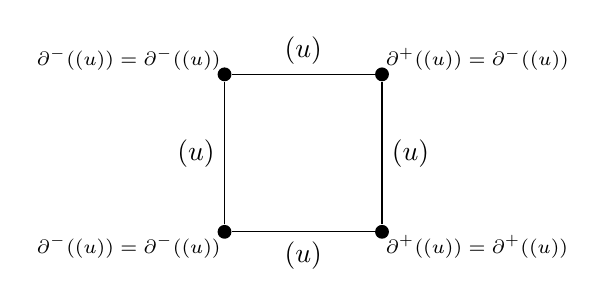
\begin{tikzpicture}[auto,scale=2,color=black]
\node(UL) [fill,circle,inner sep=0pt,minimum size=5pt,label={[label distance=-.2cm]above left: 
	{\scriptsize{$\partial^- (\upperf (u)) = \partial^- (\leftf (u))$}}}] at (0,1) {};
\node(UR) [fill,circle,inner sep=0pt,minimum size=5pt,label={[label distance=-.2cm]above right: 
	{\scriptsize{$\partial^+ (\upperf (u)) = \partial^- (\rightf (u))$}}}] at (1,1) {};
\node(BL) [fill,circle,inner sep=0pt,minimum size=5pt,label={[label distance=-.2cm]below left:
	{\scriptsize{$\partial^- (\upperf (u)) = \partial^- (\leftf (u))$}}}] at (0,0) {};
\node(BR) [fill,circle,inner sep=0pt,minimum size=5pt,label={[label distance=-.2cm]below right:
	{\scriptsize{$\partial^+ (\lowerf (u)) = \partial^+ (\rightf (u))$}}}] at (1,0) {};
\draw (UL) -- (UR) node [above, midway] {$\upperf(u)$};
\draw (UR) -- (BR) node [right, midway] {$\rightf(u)$};
\draw (BR) -- (BL) node [below, midway] {$\lowerf(u)$};
\draw (BL) -- (UL) node [left, midway] {$\leftf(u)$};
\end{tikzpicture}
\caption{A square $u \in D_2$ and its iterated faces.}
\end{figure}











